\chapter{Frontend Electronic of the Scintillating Fiber Hodoscope}\label{cha:frontend}

%table of slow control register has to be checked
%DAC output voltage (\SI{5}{\volt}) has to be understood

\section{Overview of the Frontend Electronics}
\begin{figure}[h]
    \centering
    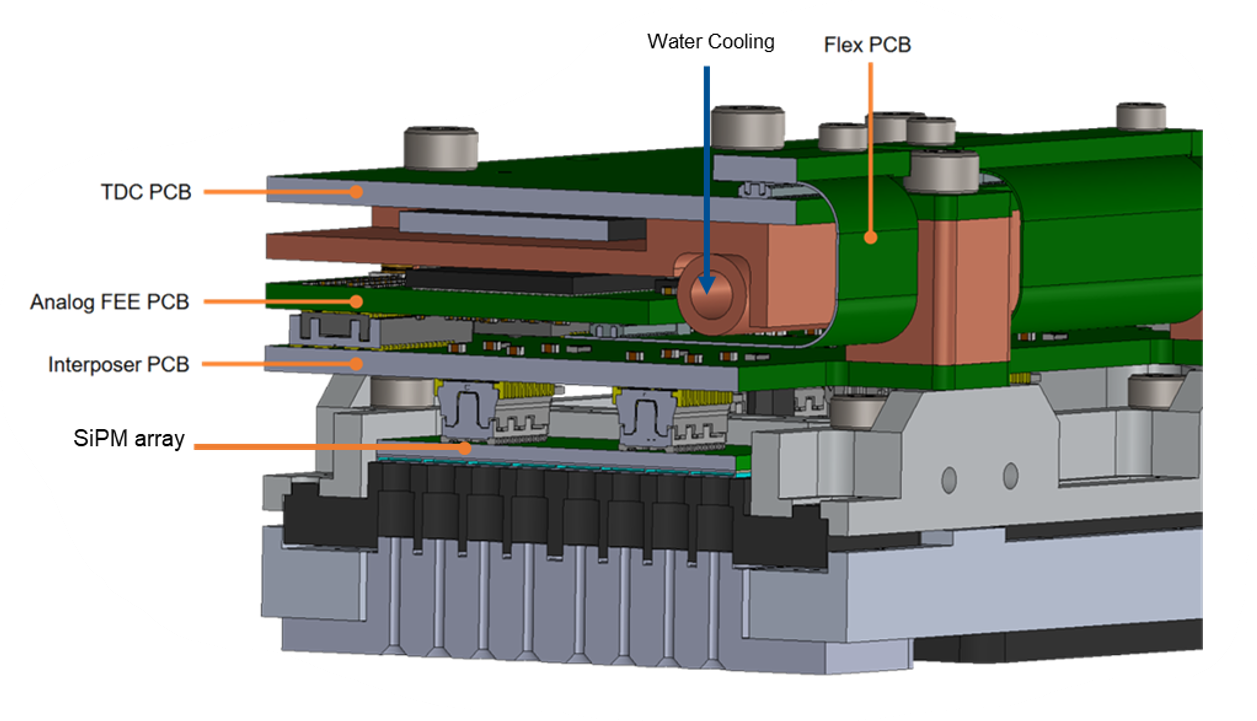
\includegraphics[width=0.9\textwidth]{FrontendAngluarview.png}
    \caption{Sideview of the frontend electronics that will be attached on the sides of the SFH, the fiber holders will be attached to the fibers.\autocite{InternalcommunicationKarl} }
    \label{fig:SideviewModelElectronics}
    \end{figure}
\subsection{Proccesing of the SFH Signal}
The frontend electronics of the scintillating fiber hodoscope process the signals from the scintillating fibers.
They can be attached on all four sides of the SFH, as can be seen in Figure \ref{SFHpicture}.
The fibers are connected to the fiber holders on both ends as shown in Figure \ref{fig:SideviewModelElectronics}. 
There are in total 768\autocite{Amber2022Status} fibers per SFH. Since both ends produce an electric signal,
a total of 1546 signals have to be proccesed. This would require a total of 48 Citiroc1A ASICs, spread over 8 frontend electronics units. 
To mittigate the cost of the frontend electronics, as well as limit the amount of data that has to be proccesed, a mirrored setup is planed.
In this setup only one end of the fibers is connected to the SiPM array, while the other end is mirrored. This would reduce the amount of reqiured frontend electronics units to 4.\autocite{InternalcommunicationKarl}
\newline
The incoming photons are transformed into electric signals by the SiPM arrays.
The SiPM signals are then transmitted to the analog frontend electronics (FEE) PCB by the interposer PCB also shown in Figure \ref{fig:SideviewModelElectronics}.
\newline
The FEE PCB and the iFTDC are the two main components of the frontend electronics, as shown in Figure \ref{fig:SideviewModelElectronics}, and are connected over three flex PCBs as well as plug connectors.
The whole setup is cooled by a water cooling system and is designed in a way that minimizes its size in order to reduce the amount of material in the beamline.\autocite{InternalcommunicationKarl}    
\subsection{The Analog Frontend Electronics (FEE) PCB}
\begin{figure}[H]
    \centering
    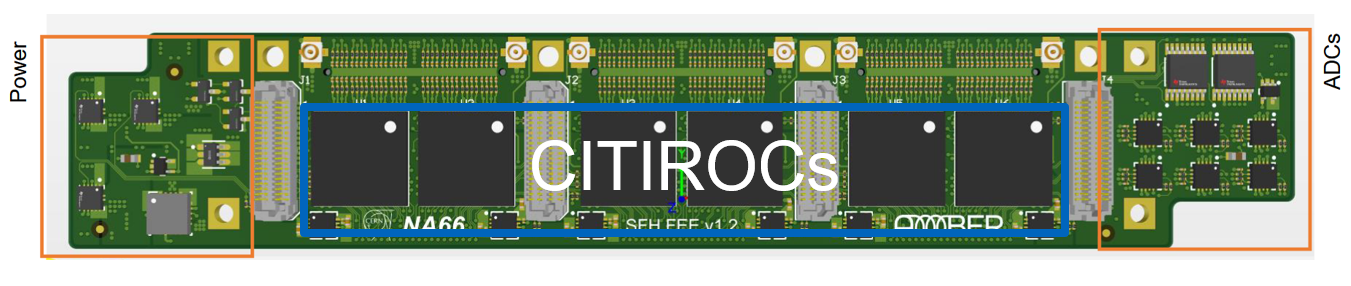
\includegraphics[width=0.6\textwidth]{beschrifteterFEE.png}
    \caption{The analog frontend electronics (FEE) PCB with the six Citiroc1A ASICs, on the left side the power supply and on the right side ADCs for temporary readout, inorder to test the SFH.
    The output of the Citiroc1A ASICs is transmitted to the iFTDC over three flex PCBs.\autocite{InternalcommunicationKarl}}
    \label{fig:FEE}
\end{figure}
The analog frontend electronics (FEE) PCB, shown in Figure \ref{fig:FEE}, together with the iFTDC forms the heart of the frontend electronics.
The FEE PCB incorporates six Citiroc1A ASICs, which are designed to amplify and process the signals from the SiPM arrays.
Each Citiroc1A ASIC handles 32 signals. The output of the ASICs is then transmitted to the iFTDC over three flex PCBs.
Two Citirroc1A ASICs are each controlled by one Artix-7 FPGA located on the iFTDC.\autocite{InternalcommunicationIgor}
\newline
Currently for prototype testing the SFH is read out by the ADCs on the FEE PCB, as is illustrated on the right side of the FEE PCB in Figure \ref{fig:FEE}, but the final setup will use the iFTDC for the readout of the SFH.\autocite{InternalcommunicationKarl} 
\subsection{The iFTDC}\label{sec:iFTDC}
\begin{figure}[H]
    \centering
    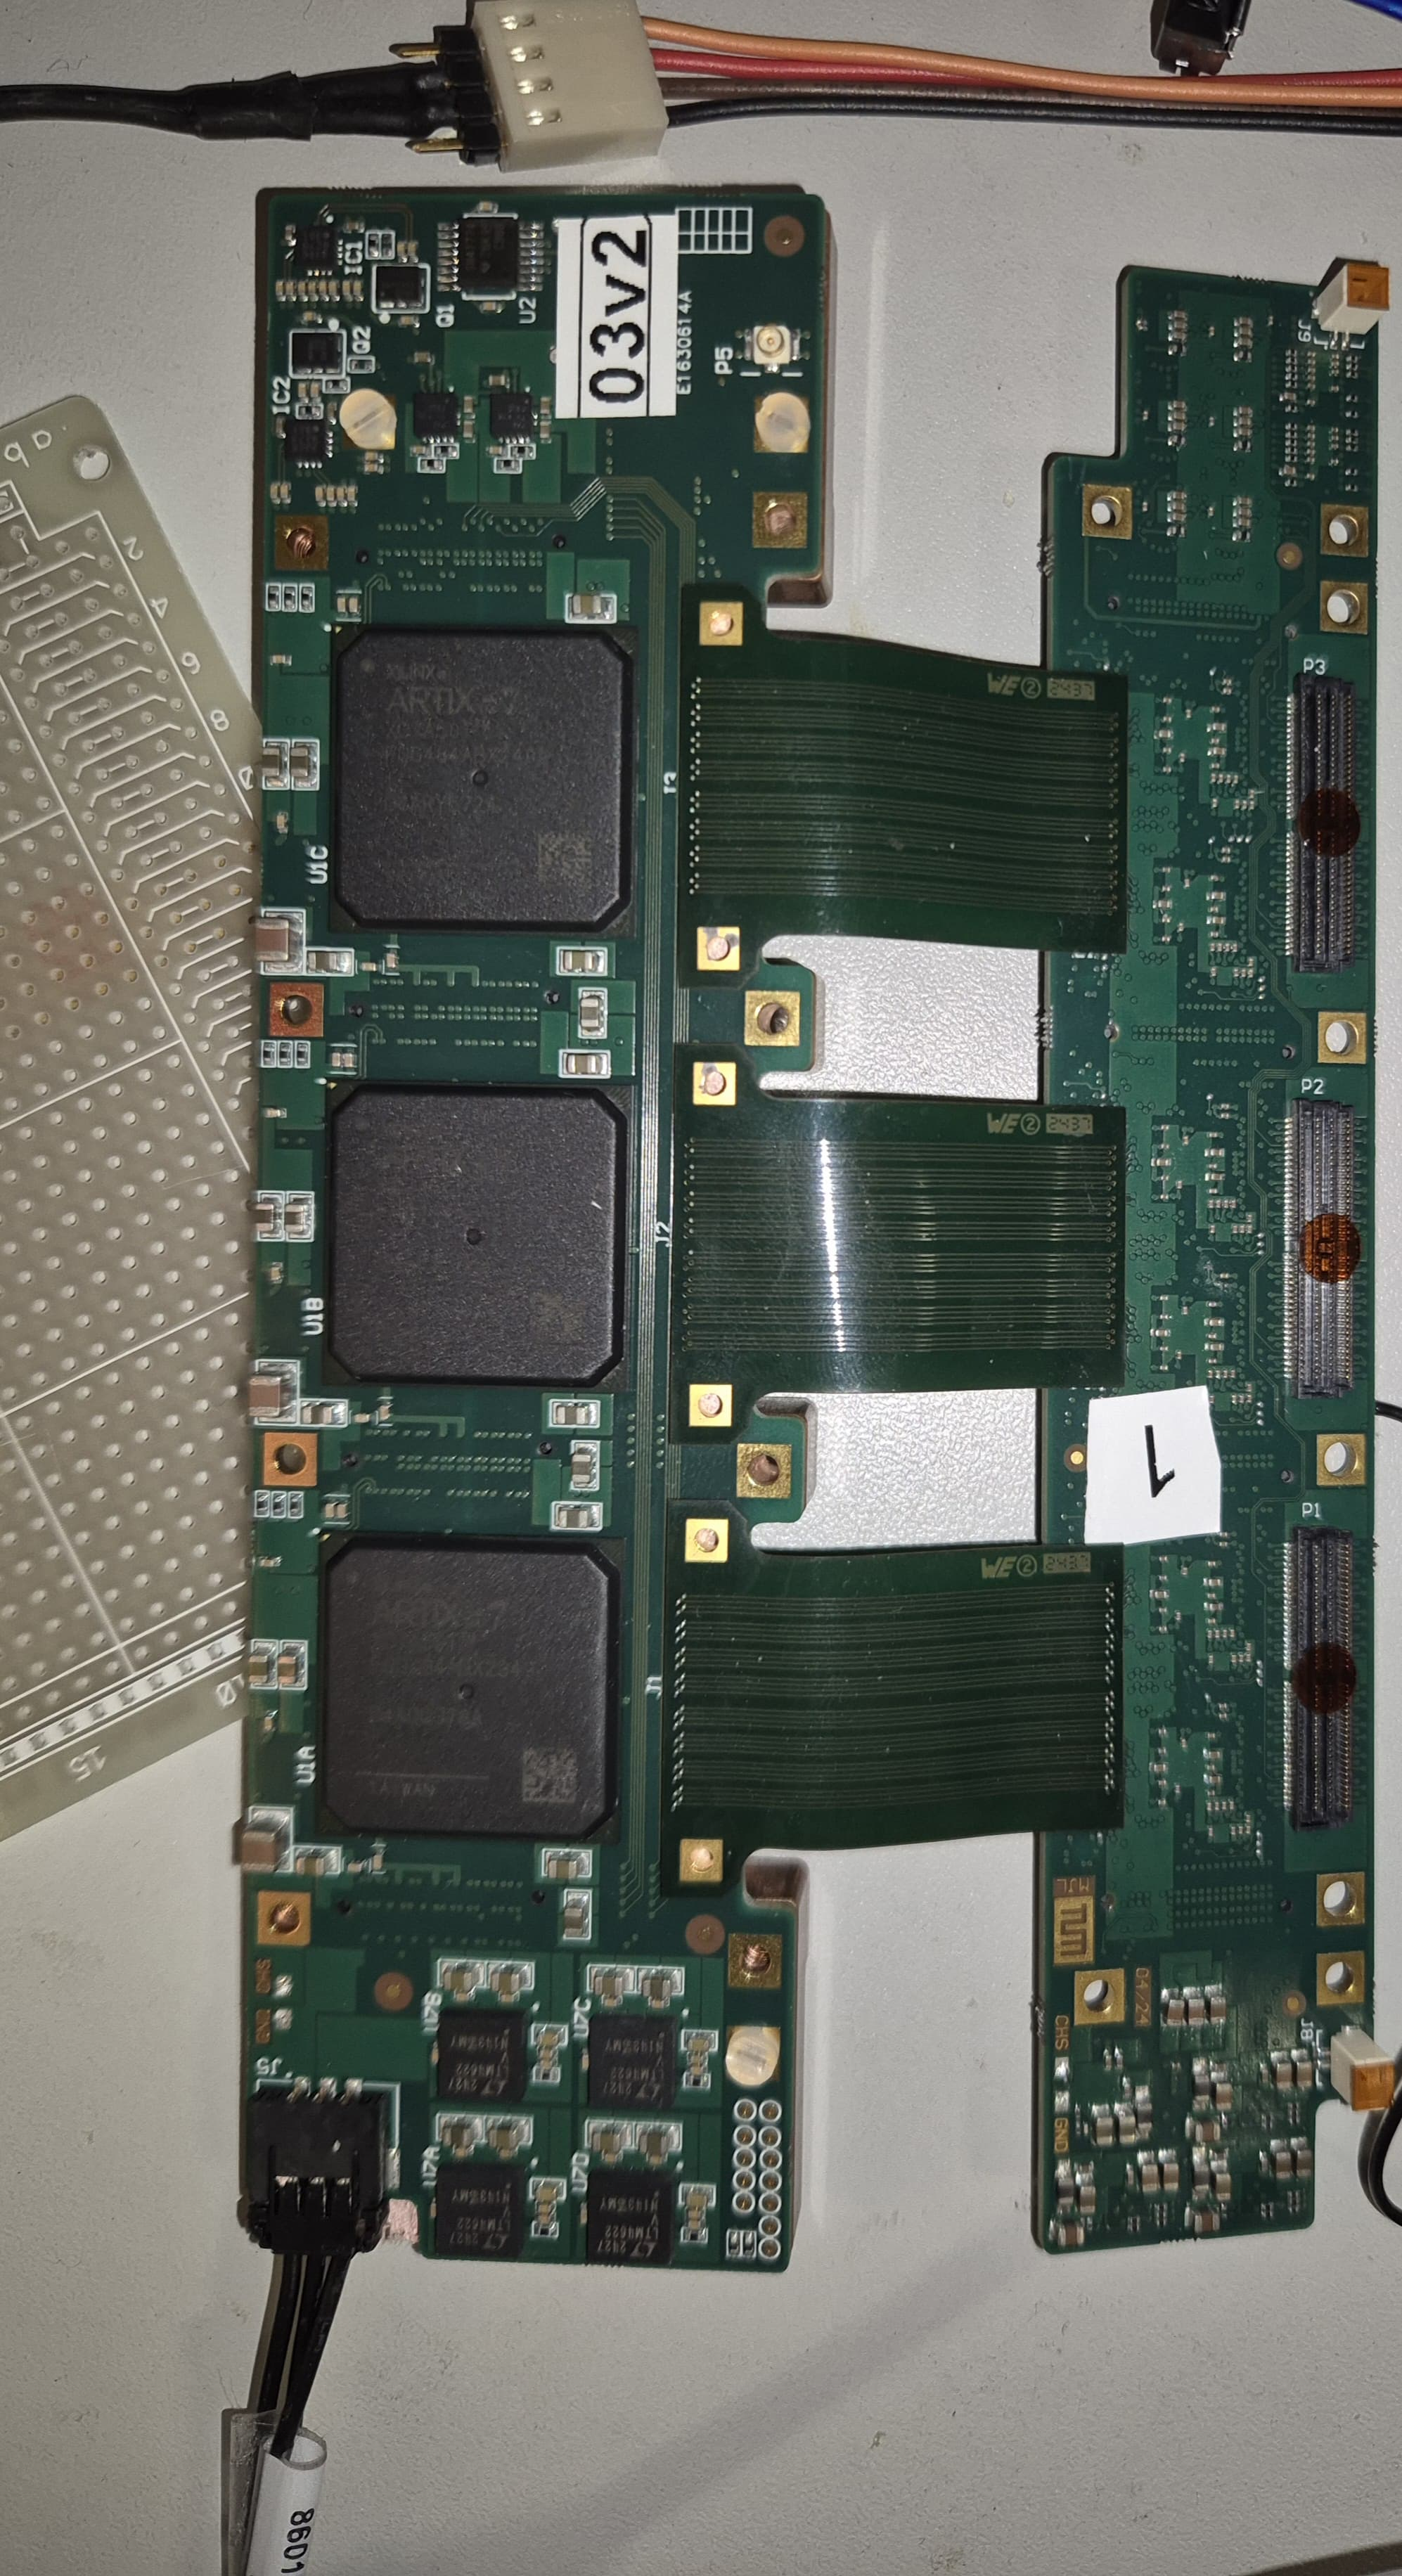
\includegraphics[width=0.5\textwidth]{WhatsApp Bild 2024-12-06 um 12.54.12_a1c66d92.jpg}
    \caption{The iFTDC with three Artix-7 FPGA, the three flex PCBs that connect the iFTDC with the FEE PCB and the connected power suply.}
    \label{fig:iFTDC}
\end{figure}

The iFTDC, depicted in Figure \ref{fig:iFTDC} is a FPGA based time-to-digital converter. It consists of three Artix-7 FPGA, who each control two Citiroc1A ASICs.
The FPGA handels the readout as well as the configuration of the Citiroc1A ASICs\autocite{InternalcommunicationIgor}.
\newline
The FPGAs are programmed via jtag and connected to the controling computer via ethernet.
\section{The Citiroc1A ASIC}
The Citiroc1A ASIC is a frontend application-specific integrated circuit developed by Weeroc for the readout of SiPM detectors.
It allows for the readout of 32 channels and is sensitive to $\frac{1}{3}$ of a photoelectron.\autocite{datasheetCITIROC}
\newline
The Citiroc1A ASIC is controlled and readout by the Artix-7 FPGAs on the iFTDC, each FPGA controlling two Citiroc1A ASICs.\autocite{InternalcommunicationIgor}
The focus of this thesis is the development of the FPGA firmware for the control of the Citiroc1A ASICs,
but a provesional readout firmware for testing the configuration of the Citiroc1A will also be developed.
\subsection{Signal Proccesing of the Citiroc1A}
\begin{figure}[h]
    \centering
    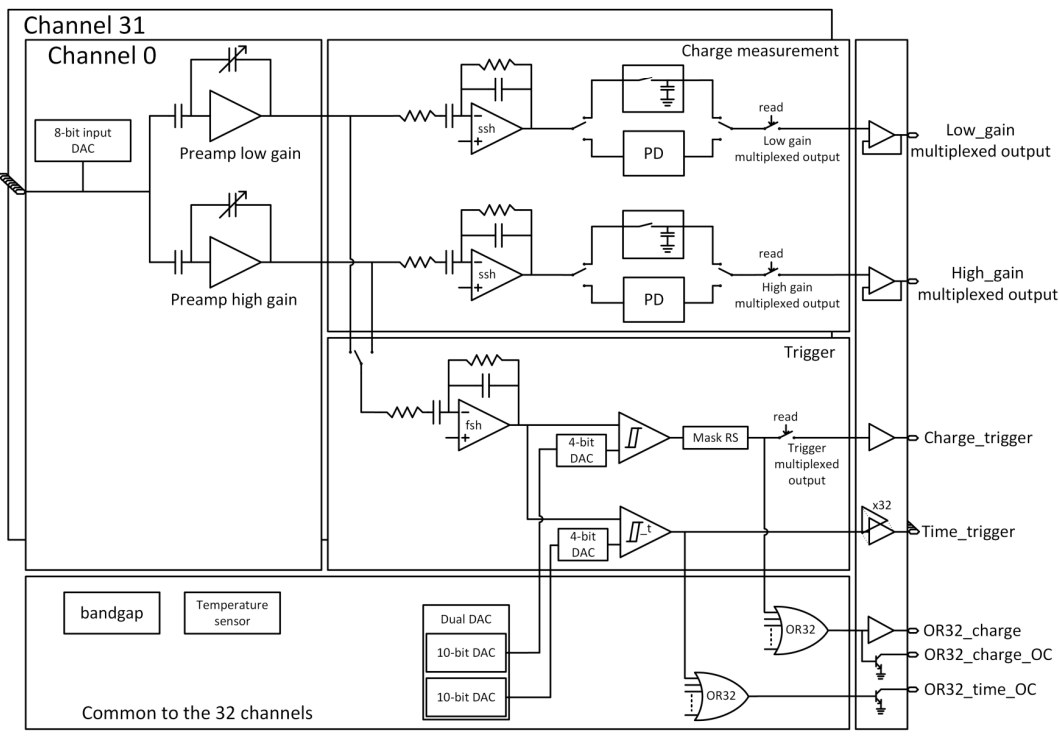
\includegraphics[width=0.8\textwidth]{TRIGER.PNG}
    \caption{General ASIC block scheme of the Citiroc1A.\autocite{datasheetCITIROC}}
    \label{fig:CITIROC1A_TRIGEER}
\end{figure}

\begin{figure}[h]
    \centering
    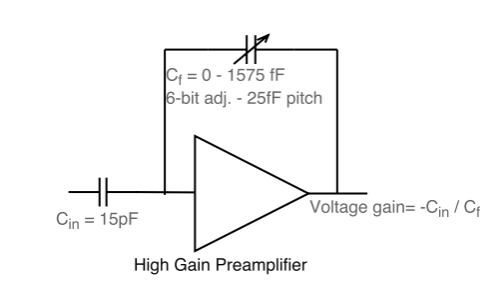
\includegraphics[width=0.8\textwidth]{HighGain.PNG}
    \caption{High gain amplification of the Citiroc1A. The gain is adjustable from 0 to \SI{1575}{\femto\farad} in \SI{25}{\femto\farad} steps.\autocite{datasheetCITIROC}}
    \label{HighGain}
\end{figure}
The general block scheme of the Citiroc1A is shown in Figure \ref{fig:CITIROC1A_TRIGEER}.
\newline
The Citiroc1A allows for the fine tuning of the SiPM bias voltage for each channel via the 8-bit input DAC.
\newline	
The input signals are amplified with a variable high or low gain, configurable for every channel as depicted in Figure \ref{HighGain}. 
The PRM experiment requires the maximal high gain of 62.\autocite{InternalcommunicationIgor}
\newline
The amplified signals are then shaped by either the slow (ssh) or fast shaper (fsh) as shown in Figure \ref{fig:CITIROC1A_TRIGEER}. 
The fast shaper is used for the PRM experiment, since it has a \SI{15}{\nano\second} peaking time and a better time resuliton, which is needed for the time precision of the SFH.\autocite{datasheetCITIROC}
\newline
The ASIC has two discriminators, the charge discriminator and the time discriminator. In this thesis we will only look at the time discriminator,
since it provides the time information.
The time discriminator threshold is adjustable via a 10 bit dac for all channels and an additional 4 bit dac for every individual channel as shown in Figure \ref{fig:CITIROC1A_TRIGEER}\autocite{datasheetCITIROC}.


\section{Configuration of the Citiroc1A}\label{sec:configuration}
\begin{figure}[h]
    \centering
    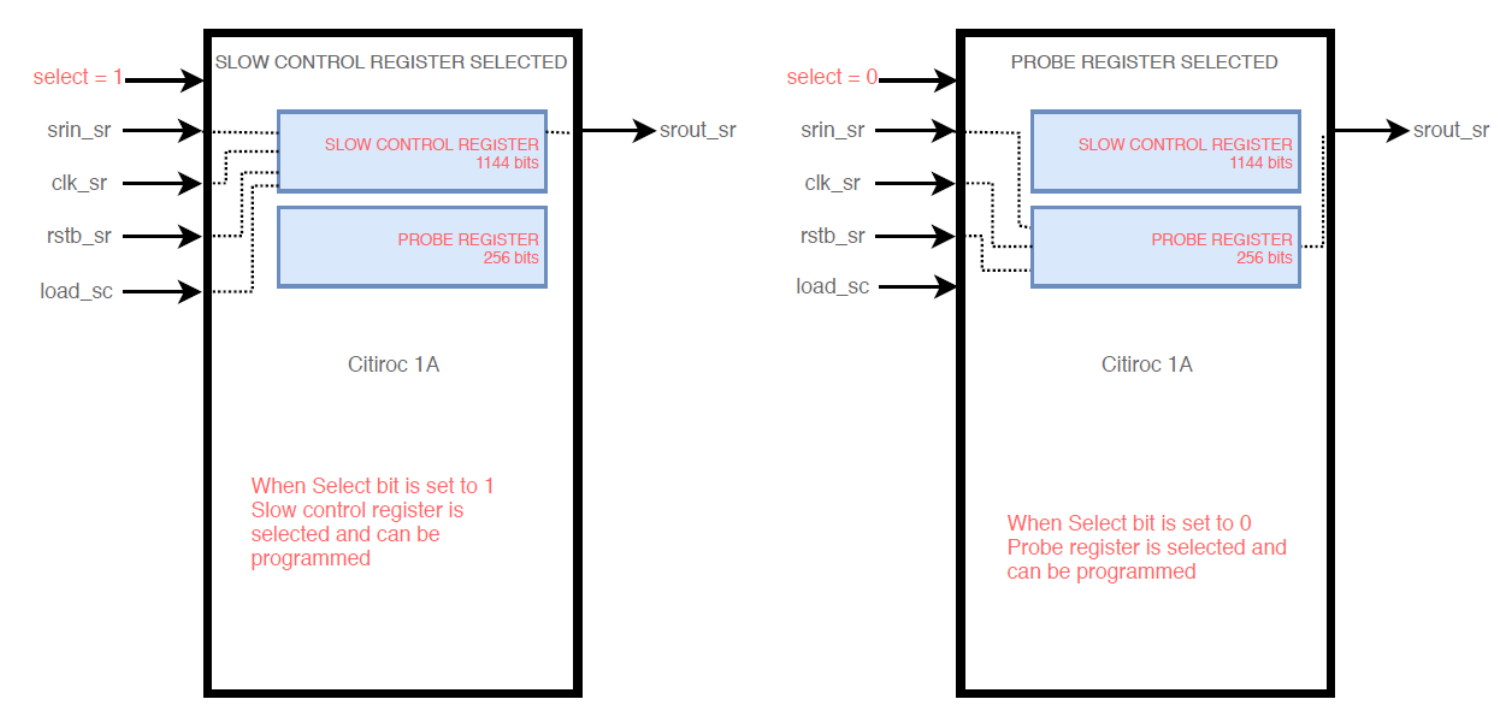
\includegraphics[width=0.8\textwidth]{CitirocConfigHighqual.png}
    \caption{The two configurable registers of the Citiroc1A are selected using the \textcolor{red}{Select} signal. 
    The FPGA communicates with the Citiroc1A through the signals \textcolor{red}{Clk\_sr}, \textcolor{red}{Rstb\_sr}, 
    \textcolor{red}{Srin\_sr}, and \textcolor{red}{Load\_sr}, while the \textcolor{red}{Srout} signal is sent back from the Citiroc1A to the FPGA for verification.\autocite{datasheetCITIROC}}
    \label{fig:CITIROC1A_config}
\end{figure}
The configuration of the Citiroc1A is achievied by the FPGA via the five signals shown in Figure \ref{fig:CITIROC1A_config}.
The \textcolor{red}{Select} signal allowes the choice between configuring the slow control, for \textcolor{red}{Select} = 1  or the probe register, for \textcolor{red}{Select} = 0.\autocite{datasheetCITIROC}

\subsection{The Slow Control Register}

\begin{figure}
    \centering
    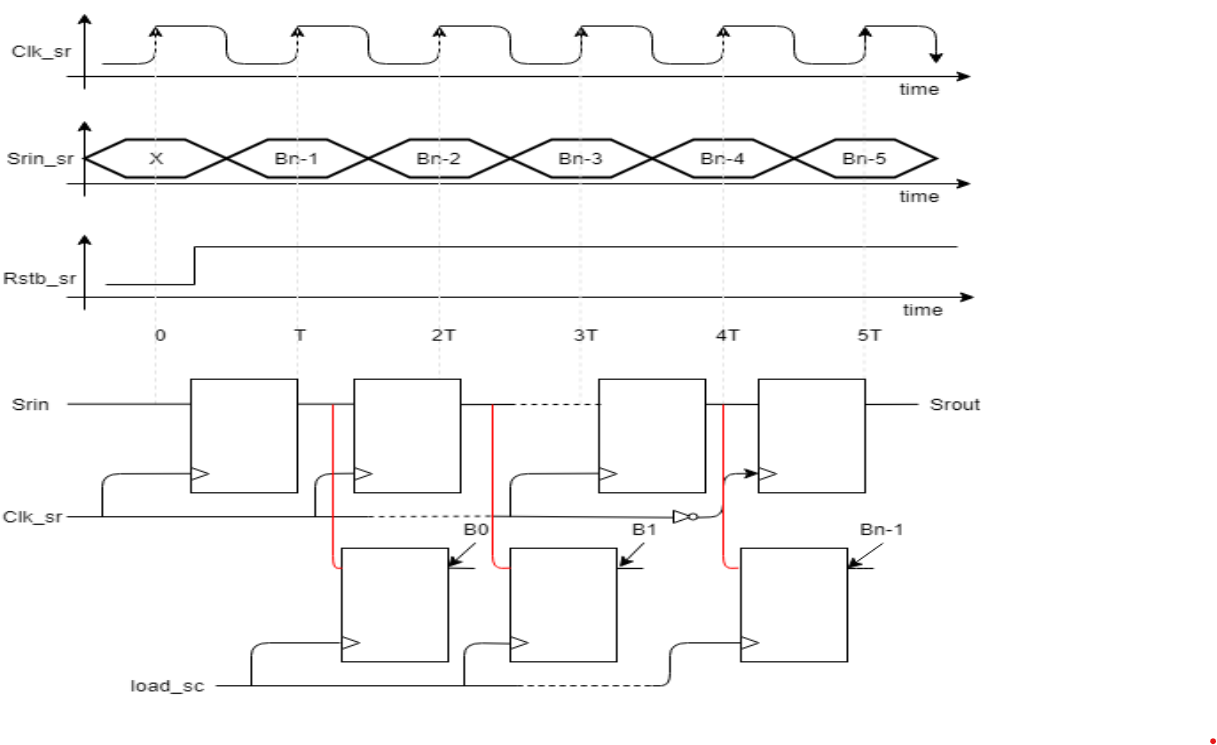
\includegraphics[width=0.8\textwidth]{BitwriteSlowControl.png}
    \caption{The slow control chronogram, depicting the bitstream writing process controled by  \textcolor{red}{Clk\_sr} the clock signal and  \textcolor{red}{Srin\_sr} the data signal. A rising edge of \textcolor{red}{Load\_sr} is required,
     after successful verification with the \textcolor{red}{Srout} signal to load the slow control register.\autocite{datasheetCITIROC}}
    \label{fig:CITIROC1A_writing_bitstream}
\end{figure}
The slow control register is used to set values for internal variables like the high gain for a channel or the time discriminator threshold.
It also allowes for the FPGA to turn of spesific stages of the Citiroc1A, such as the slow shaper or the time discriminator.
The register is 1144 bits long. A full list of all the register that can be set is shown in Table \ref{tab:slow_control_register} in Appendix \ref{cha:Citiroc1A_register}.
\newline
The process of writing the bitstream into the slow control register by the FPGA is illustrated in Figure \ref{fig:CITIROC1A_writing_bitstream}.
\newline
The \textcolor{red}{Rstb\_sr} signal is an asynchronous active-high reset for the serial register, applying to both the slow control and probe register. 
\newline
The FPGA processes the bitstream sequentially, starting with the least significant bit (LSB).
The first bit of the bitstream to enter the serial register will be the last bit of the slow control register.
Each bit is sent on the \textcolor{red}{Srin\_sr} signal in coordination with a rising edge of the \textcolor{red}{Clk\_sr} clock signal.
\newline
The \textcolor{red}{Load\_sr} signal is used to load the bitstream into the slow control register. After all bits have been sent to the Citiroc1A,
a rising edge on \textcolor{red}{Load\_sr} is required to load the slow control register.
\newline
The \textcolor{red}{Srout} signal is sent back from the Citiroc1A to the FPGA for bitstream verification.
Only after the FPGA has sent the full bitstream twice, does the \textcolor{red}{Srout} signal take on the value of the bitstream, since the \textcolor{red}{Srout} signal is shifted by the length of the bitstream.\autocite{datasheetCITIROC}
One should only set the rising edge of the \textcolor{red}{Load\_sr} signal after verifying that the \textcolor{red}{Srout} signal takes on the correct values.

\subsection{The Probe Register}\label{sec:probe_register}
\begin{figure}[H]
    \centering
    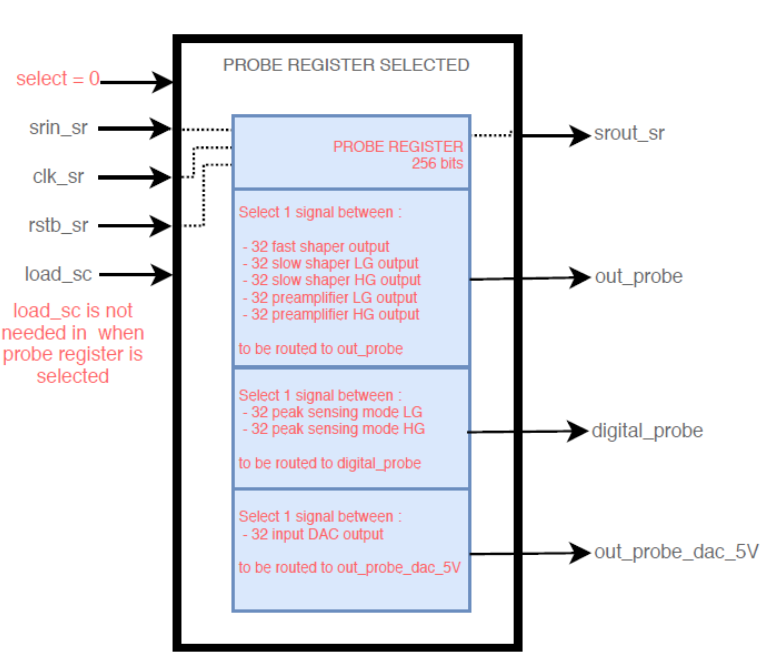
\includegraphics[width=0.8\textwidth]{ProbeRegister.png}
    \caption{Scheme block of internal probing system, allowing the routing of internal signals to probe pins for debugging purposes. It is configured via the probe register.\autocite{datasheetCITIROC}}
    \label{fig:CITIROC1A_proberegiseter}
\end{figure}
The probe register is used for routing internal signals to several output pins for debugging purposes.
It's functionality is ilustrated in Figure \ref{fig:CITIROC1A_proberegiseter}.
The register consists of 256 bits and is written the same way as the slow control register,
 with the difference that the bits are directly written into the Citiroc1A without requiring a rising edge on \textcolor{red}{Load\_sc}.\autocite{datasheetCITIROC}
\newline
 The full list of all the register that can be set in the probe register is shown in Table \ref{tab:probe_register_tab} in Appendix \ref{cha:Citiroc1A_register}.
\newline
The internal signals for each channel that can be routed to the output pins are shown in Table \ref{tab:probe_register}. 
 \begin{table}[H]
    \centering
    \begin{tabular}{@{}lll@{}}
    \toprule
    \textbf{Signal Source} & \textbf{Description}                   & \textbf{Output Pin}        \\ \midrule
    High and low gain preamplifier, & Outputs of preamplifiers and shapers & \texttt{out\_probe}        \\
    slow and fast shapers                                                   &                          \\ \midrule
    \texttt{PeakSensing\_modeb\_LG} & Internal peak-sensing signal for low gain & \texttt{digital\_probe}    \\
    \texttt{PeakSensing\_modeb\_HG} & Internal peak-sensing signal for high gain & -    \\ \midrule
    Output of input DAC            & DAC output voltage (\SI{5}{\volt})  & \texttt{out\_probe\_dac\_5\_V} \\ \bottomrule
    \end{tabular}
    \caption{Internal signal routing to output pins for each channel.}
    \label{tab:probe_register}
\end{table}
Only one signal can be routed to each output pin at a time, without potentially causing a short circuit.\autocite{datasheetCITIROC}









 

